\documentclass{article}
\usepackage{amsmath,amssymb}
\usepackage[T1]{fontenc}
\usepackage[utf8]{inputenc}
\usepackage{textcomp}
\newcommand{\midtilde}{\raisebox{-0.25\baselineskip}{\textasciitilde}}
\usepackage{graphicx}
\usepackage{float}
\graphicspath{ {./images/} }

\begin{document}

\section*{Bayesian network: example}
\begin{figure}[H]
 \centering 
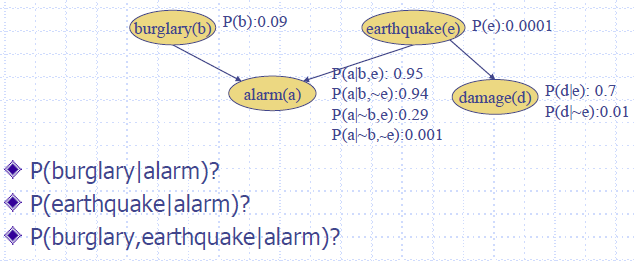
\includegraphics[scale=0.65]{images/alarm.png} 
 \caption{Bayesian network: example}
 \label{fig:b-net-example}
\end{figure}
Artur's solution:\\
Who can we find p(a)? \\
\begin{align*}
p(a) & = p(a,b) + p(a,\midtilde b) \\
Further: \\
p(a,b) & = p(a,b,e) + p(a,b,\midtilde e) \\ 
p(a,b,e) & = p(a,b,e,d) + p(a,b,e,\midtilde d) \\
and \\
p(a,b,\midtilde e) & = p(a,b,\midtilde e,d) + p(a,b,\midtilde e,\midtilde d) \\
\\
p(a,\midtilde b) & = p(a,\midtilde b,e) + p(a,\midtilde b,\midtilde e) \\ 
p(a,\midtilde b,e) & = p(a,\midtilde b,e,d) + p(a,\midtilde b,e,\midtilde d) \\
and \\
p(a,\midtilde b,\midtilde e) & = p(a,\midtilde b,\midtilde e,d) + p(a,\midtilde b,\midtilde e,\midtilde d) \\
\end{align*}
These are all of the values we need to find. \\
Let's start with the basic equation
\begin{equation}
    p(a) = p(a,b) + p(a,\midtilde b) \label{eq1}
\end{equation}
We need to find $p(a,b)$ and $p(a,\midtilde b)$ which is turn we need to find $p(a,b,e)$ and $p(a,b,\midtilde e)$\\
So,
\begin{equation}
    p(a,b,e) = p(a,b,e,d) + p(a,b,e,\midtilde d) \label{eq2}
\end{equation}
\begin{align*}
  p(a,b,e,d) & = p(a|b,e)p(b)p(e)p(d|e) \\
  & = 0.95*0.09*0.0001*0.7 \\
  & = 0.000005985 \\
\end{align*}
And,
\begin{align*}
  p(a,b,e,\midtilde d) & = p(a|b,e)p(b)p(e)p(\midtilde d|e) \\
  & = 0.95*0.09*0.0001*[1-p(d|e)] \\
  & = 0.95*0.09*0.0001*0.3 \\
  & = 0.000002565 \\
\end{align*}
Plugging these 2 values back into Equation \ref{eq2},
\begin{align*}
p(a,b,e) & = p(a,b,e,d) + p(a,b,e,\midtilde d) \\
p(a,b,e) & = 0.000005985 + 0.000002565 \\
p(a,b,e) & = 0.00000855 \\
\end{align*}
Next step is to find $p(a,b,\midtilde e)$ (Note typo in pdf)
\begin{equation}
    p(a,b,\midtilde e) = p(a,b,\midtilde e, d) + p(a,b,\midtilde e,\midtilde d) \label{eq3}
\end{equation}
First
\begin{align*}
    p(a,b,\midtilde e, d) & = p(a|b,\midtilde e)p(b)p(\midtilde e)p(d|\midtilde e) \\
    & = 0.94*0.09*0.9999*0.01 \\
\end{align*}
\begin{equation}
    = 0.00084592 \label{eq4}
\end{equation}
And, (note typo in original text should read $1 - p(\midtilde d|\midtilde e)$ though value is correct).
\begin{align*}
    p(a,b,\midtilde e, \midtilde d) & = p(a|b,\midtilde e)p(b)p(\midtilde e)p(\midtilde d|\midtilde e) \\
    & = 0.94*0.09*0.9999*[1-p(\midtilde d|e)] \\
    & = 0.94*0.09*0.9999*0.99 \\
\end{align*}
\begin{equation}
    = 0.0837 \label{eq5}
\end{equation}
From equation \ref{eq1} we now have $p(a,b)$
\begin{align*}
    p(a,b) & = p(a,b,e) + p(a,b,\midtilde e) \\
    & = 0.00000855 + [ eq. 4 + eq. 5 ]
    & = 0.00000855 + 0.00084592 + 0.0837 \\
    p(a,b) = 0.0846
\end{align*}
Using the same approach above, we need to find p(a,\midtilde b) for Eqn \ref{eq1}
\begin{equation}
    p(a,\midtilde b) = p (a,\midtilde b, e) + p(a, \midtilde b, \midtilde e) \label{eq6}
\end{equation}
from \ref{eq6},
\begin{equation}
    p(a, \midtilde b, e) = p(a,\midtilde b, e, d) + p(a,\midtilde b, e, \midtilde d) \label{eq7}
\end{equation}
To find the 2 parts of \ref{eq7}
\begin{align*}
    p(a,\midtilde b, e, d) = p(a|\midtilde b, e) p(\midtilde b) p(e)
\end{align*}



Solution excluding damage:
\begin{align*}
p(b|a) ? & \\
p(e|a) ? & \\
p(b,e|a) ? & \\
p(a) & = p(a,b) + p(a,e) \\
p(a,b) & = p(a,b,e) + p(a,b,\midtilde e) \\
p(a,b,e) & = p(e)p(b)p(a|b,e) = 0.0001*0.09*0.95 = 0.00000855 \\
p(a,b,\midtilde e) & = p(\midtilde e)p(b)p(a|b,\midtilde e) = 0.9999*0.09*0.94 = 0.0846\\
p(a,b) & = p(a,b,e) + p(a,b,\midtilde e) = 0.00000855 + 0.0846 = 0.0846 \\
p(a,\midtilde b,e) & = p(e)p(\midtilde b)p(a|\midtilde b,e) = 0.0001*0.91*0.29 = 0.00002639 \\
p(a,e) & = p(a,b,e) + p(a,\midtilde b,e) = 0.00000855 + 0.00002639 = 0.00003494 \\
p(a) & = p(a,b) + p(a,e) =  0.0846 + 0.00003494 =  0.0846\\
p(b|a) & = \frac{p(a,b)}{p(a)} = \frac{0.0846}{0.0846} = 1\\
p(e|a) & = \frac{p(a,e)}{p(a)} = \\
p(b,e|a) & = \frac{p(e)p(b)p(a|b,e)}{p(a)} \\
\end{align*}
Including damage:
\begin{align*}
p(b|a) ? & \\
p(e|a) ? & \\
p(b,e|a) ? & \\
p(a) & = p(a,b) + p(a,e,d) \\
\end{align*}
\end{document}